\documentclass{sig-alternate-05-2015}

\usepackage{multirow}
\DeclareMathOperator*{\argmin}{argmin}
\DeclareMathOperator*{\argmax}{argmax}

\begin{document}

%\setcopyright{}
%\doi{}
%\isbn{}
%\conferenceinfo{}
%\acmPrice{\$15.00}
% Author Metadata

\title{Trajectory Recommendation}

%\numberofauthors{}
%\author{
%\alignauthor
%\alignauthor
%\alignauthor
%}

\maketitle

%\begin{abstract}

%%!TEX root = main.tex

The problem of recommending tours to travellers is an important and broadly studied area.
Suggested solutions include various approaches of points-of-interest (POI)
recommendation and route planning.
We consider the task of recommending a sequence of POIs 
%as a tour to travellers
, that simultaneously uses information about POIs and routes.
Our approach unifies the treatment of various sources of information
by representing them as features in machine learning algorithms, enabling us to
learn from past behaviour. %without specialised treatment of spatial, temporal or social information.
Information about POIs are used to learn a POI ranking model
that accounts for the start and end points of tours.
Data about previous trajectories are used for learning transition patterns between POIs that
enable us to recommend probable routes.
In addition, a probabilistic model is proposed
%and a Structured Support Vector Machine are used
to combine the results of POI ranking as well as the POI-POI transitions.
We propose a new F$_1$ score on pairs of POIs
that capture the order of visits.
Empirical results show that our approach improves on
recent methods, and demonstrate that
combining points and routes enables better trajectory recommendations.


%\end{abstract}

% The code below should be generated by the tool at
% http://dl.acm.org/ccs.cfm
% Please copy and paste the code instead of the example below. 

%\printccsdesc
%\keywords{}

%\section{Introduction}
\label{sec:introduction}
Location based information sharing services provided by online social media
(e.g. Facebook, Twitter, Flickr etc) generated a lot of data with geographical information,
together with time-tamps and user tags, makes it possible to generate massive trajectories.
There is great opportunity to explore visiting patterns from these trajectory data by leveraging POI properties
as well as transition patterns between different POIs, which leads a way to recommend high quality trajectories to tourists.

In this work, we propose to utilize learning to rank to capture the properties of POIs as well as a Markov Chain to
represent the transition patterns between POIs, furthermore, we factorize the transition probabilities between POIs
according to several POI features to deal with data sparsity.
We combine the results of learning to rank and the factorized Markov Chain using both a probabilistic model and a structured
support vector machine, and evaluate the quality of POIs in recommended trajectories in terms of trajectory F$_1$-score\cite{ijcai15} and
adapt Kendall's $\tau$ coefficient\cite{kendalltau} to measure the quality of the recommended POI visiting orders in trajectories.
Experimental results on four trajectory datasets show performance improvements over the state-of-the-art methods and
reveal many interesting properties of trajectories in different datasets.


novel points:

(1) joint optimization of point preference and route plan;
(2) feature-driven, incorporates information about time, location, POI categories and behavior history
(3) strong performance compared to IJCAI 2015. we can also quantify the contribution from both point ranking and routing.
(4) F1 on pairs.

%\section{Related Work}
\label{relatedwork}
% IJCAI'15
\cite{ijcai15} formulated trajectory recommendation as a Orienteering problem,
by optimizing an objective which was a composite of total POI popularity of the recommended trajectory
and the total user interest of the categories of the recommended POIs, the interest of a user at a specific 
category of POI was modelled as the summation of ratios of the visited duration by the user over the average 
duration of all visitors at all POIs of that category. The actual time consumption in a real trajectory, including
both the time spent traveling from one place to another and the time spent at all POIs of the real trajectory,
was used to constrain the time consumed in the recommended trajectory, in addition, with a start place and a 
destination specified, they recommended a trajectory by solving the Orienteering problem using integer programming.
%
The authors formulated a integer programming to solve the itinerary recommendation problem for traveller, the approach based on an essential concept that if a user is more interested in a certain category (e.g. park, museum, etc) of POIs, his/her visit duration should be longer than average in general.


% WSDM'14
\cite{wsdm14} proposed a framework to recommend customized tours (venue's type, visiting order, budget constraint and user statisfaction). They investigated two variants of user statisfaction, i.e. additive benefits and attraction coverage, proved that problems using both user satisfaction functions are NP-hard (reduce TSP to these problems) firstly and then designed two algorithms to solve the two recommendation problems using dynamic programming paradigm, both the time and space complexity of the algorithms are pseudo polynomial/exponential, but they are fast here as the scale of the input in the experimental dataset is small. They also designed an ($1-\epsilon$) approximation algorithm, proposed extensions of their framework, though without evaluating both of them in experiments.
Pros:
take into account both venue's type and user's visit order
formal proof of problem hardness
designed both exact and approximate algorithms
extend framework to incorporate factors appear in real scenarios
Cons:
algorithms evaluated in experiments are still exponential, though efficient in small input scales
dataset used in experiments is not available (a part of another dataset 2010-2011 which could be requested, newer and similar datasets 2011-2012 are freely available)

\cite{tripbuilder15}

\cite{tripplanner15}

\cite{ht14}

\cite{geophoto13}

\cite{travel13}

\cite{transit15}

%!TEX root = main.tex

\secmoveup
\section{POI, Query and Transition}
\label{sec:feature}

The goal of tour recommendation is to suggest a sequence of POIs, $(p_1, \ldots, p_L)$, of length $L$ such that the user's utility is maximised. The user provides the desired start ($p_1=p_s$) and end point ($p_L=p_e$), as well as the number $L$ of POIs desired, from which we propose a trajectory through the city.
%
%In Figure~\ref{fig:threesettings}(c), an example tour is shown in blue, which starts at the POI denoted as a grey star, visits two intermediate POIs, and terminates on the fourth POI denoted as a flag. The tour of length 4 can be modelled as a sequence of directed edges in a graph containing POIs in the city as nodes.
%
The training data consists of a set of tours of varying length in a particular city.
We consider only POIs that have been visited by at least one user in the past, and
construct a graph with POIs as nodes and directed edges representing the observed transitions between pairs of POIs in tours. %a set of tours.
%The set of categories are shown in Figure~\ref{fig:poicats} in the appendix, and the popularity is defined as the number of distinct users that visited the POI\cite{ht10}.



%\subsection{POI Features and Query}
%\label{sec:poifeature}

We extract the category, popularity (number of distinct visitors)~\cite{ht10}, total number of visits and average visit duration for each POI.
POIs are grouped into $5$ clusters using K-means according to their geographical locations to reflect their neighbourhood.
%A naive approach would be to recommend the trajectory based on the popularity (number of distinct visitors)~\cite{ht10} of POIs only,
%that is we always suggest the top-$k$ most popular POIs for all visitors given the start and end location,
%and its only adaptation to a particular request is to adjust $k$ to match the desired length.
%In addition to popularity,
%we can also rank the candidate POIs based on the other three POI specific features (category, total visits and average duration).
Furthermore, since we are constrained by the fact that trajectories have to be of length $L$ and start and end at certain points, we hope to improve the recommendation by using this information.
In other words, we use the \textit{query} $q = (p_s, p_e, L)$ to construct new features by contrasting candidate POIs with $p_s$ and $p_e$.
%
For each of the POI features (category, neighbourhood, popularity, total visits and average duration),
we construct two new features by taking the difference of the feature in POI $p$ with $p_s$ and $p_e$ respectively.
For the category (and neighbourhood), we set the feature to $1$ when their categories (and cluster identities) are the same and $-1$ otherwise.
For popularity, total visits and average duration, we take the real valued difference.
Lastly, we compute the distance from POI $p$ to $p_s$ (and $p_e$) using the Haversine formula~\cite{haversine},
and also include the required length $L$.


%\subsection{Transition probabilities}
%\label{sec:transition}


\begin{figure}[t]
%\includegraphics[width=\textwidth]{fig/poi_transmat.png}
\includegraphics[width=\columnwidth]{fig/poi_transmat.png}
\caption{Transition matrices for two POI features from Melbourne: POI categories and neighborhood.
%See Section~\ref{sec:feature} for details.
}
\label{fig:transmat}\captionmoveup
\end{figure}


In addition to information about each individual POI, a tour recommendation system would benefit
from capturing the likelihood of going from one POI to another different POI. One option would be to
directly model the probability of going from any POI to any other POI, but this has several weaknesses:
Such a model would be unable to handle a new POI (one that has not yet been visited),
or pairs of existing POIs that do not have an observed transition.
Furthermore, even if we restrict ourselves to known POIs and transitions,
there may be locations which are rarely visited,
leading to significant challenges in estimating the probabilities from empirical data.

We model POI transitions using a Markov chain with discrete %factored
states by factorising the transition probability ($p_i$ to $p_j$) %from POI $p_i$ to POI $p_j$
as a product of transition probabilities between pairs of individual POI features, %(listed in Section~\ref{sec:poifeature}),
assuming independence between these feature-wise transitions.
%We directly model the transition between the category and neighbourhood of each POI as the conditional probability.
The popularity, total visits and average duration are discretised by binning
them uniformly into $5$ intervals on the log scale.
%Transition matrices of individual POI features are computed using maximum likelihood estimation.
These feature-to-feature transitions are estimated from data using maximum likelihood principle.
The POI-POI transition probabilities can be efficiently computed by taking the Kronecker product of 
transition matrices for the individual features,
and then updating it based on three additional constraints as well as appropriate normalisation.
First we disallow self-loops by setting the probability of ($p_i$ to $p_i$) to zero.
Secondly, when multiple POIs have identical (discretised) features, we distribute the probability uniformly among POIs in the group.
%%LX: this is obvious but seem worth stating for future readers
Third, we remove feature combinations that has no POI in dataset. 
Figure~\ref{fig:transmat} visualises the transition matrices for two POI features, category and neighborhood, in Melbourne.
%More details of this procedure are provided in the Appendix.

\section{Experimental Results}
\label{experiment}

\subsection{Dataset}
\label{experiment:dataset}
We experiment on trajectories data in four cities from \cite{ijcai15} that were
extracted from Yahoo! Flickr Creative Commons 100M (a.k.a. YFCC100M) dataset\cite{yfcc100m},
and trajectories data in Melbourne that was extracted from YFCC100M the same way described in \cite{ht10, ijcai15},
dataset statistics are available in table \ref{table:data:all}-\ref{table:data:nofew}.

An example of trajectory in Melbourne was shown in figure \ref{fig:traj}.

\begin{figure}
\centering
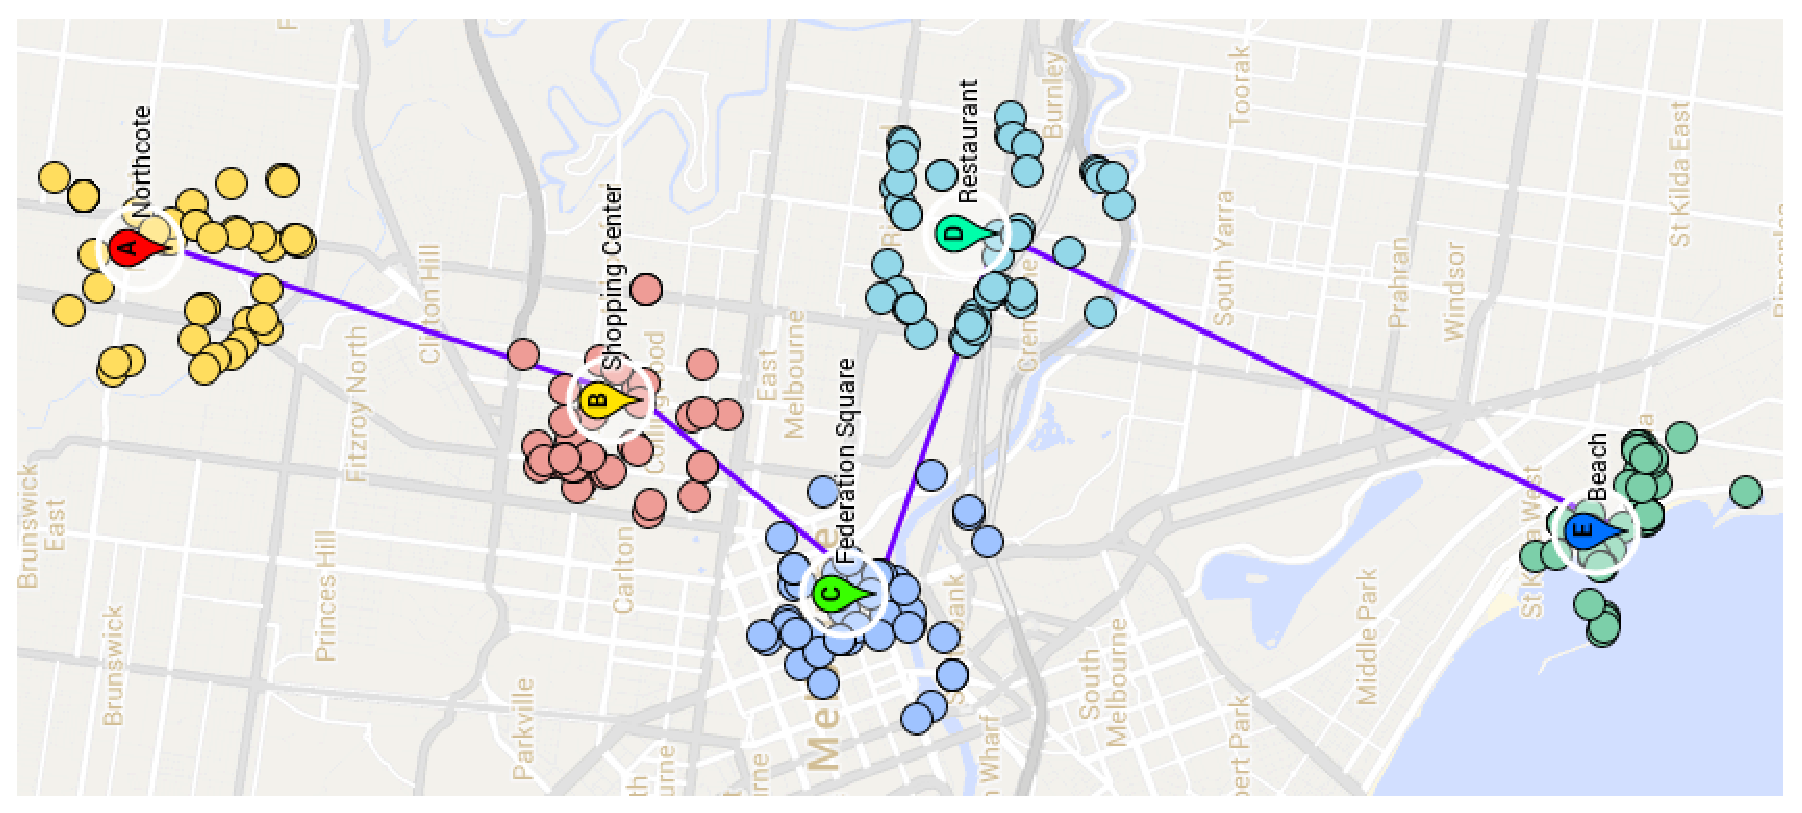
\epsfig{file=traj_eg.eps, width=3.5in}
\caption{An example of trajectory}
\label{fig:traj}
\end{figure}

\subsection{Dataset preprocess}
\label{experiment:datapreprocess}
Trajectories in all datasets are preprocessed such that no self-loops and sub-tours exist.
Concretely, after splitting a sequence of photos by a given time gap and mapping photos to a set of POIs\cite{ht10, ijcai15},
a trajectory was extracted from the result POI visiting sequence such that the order of POIs in the trajectory is the same as 
the order of the first occurrence of POIs in the visiting sequence.

\begin{table*}
\centering
\caption{Dataset of all trajectories without loops}
\label{table:data:all}
\begin{tabular}{lrrrrr} \hline
\textbf{City} & \textbf{\#POIs} & \textbf{\#Users} & \textbf{\#POI Visits} & \textbf{\#Trajectories} & \textbf{\#TotalNodes} \\ \hline
Osaka & 27 & 450 & 7,747 & 1,115 & 1,372 \\ 
Glasgow & 27 & 601 & 11,434 & 2,227 & 2,749 \\ 
Edinburgh & 28 & 1,454 & 33,944 & 5,028 & 7,853 \\ 
Toronto & 29 & 1,395 & 39,419 & 6,057 & 7,607 \\ 
Melbourne & 85 & 1,000 & 23,995 & 5,106 & 7,246 \\ 
\hline
\end{tabular}
\end{table*}

\begin{table*}
\centering
\caption{Dataset of users with more than 5 (including 5) trajectories with loops}
\label{table:data:nofew}
\begin{tabular}{lrrrrr} \hline
\textbf{City} & \textbf{\#POIs} & \textbf{\#Users} & \textbf{\#POI Visits} & \textbf{\#Trajectories} & \textbf{\#TotalNodes} \\ \hline
Osaka & 24 & 40 & 2,471 & 473 & 577 \\ 
Glasgow & 25 & 94 & 7,116 & 1,433 & 1,711 \\ 
Edinburgh & 28 & 192 & 19,149 & 2,901 & 4,420 \\ 
Toronto & 29 & 248 & 27,105 & 4,113 & 5,185 \\ 
Melbourne & 85 & 242 & 15,833 & 3,759 & 5,223 \\ 
\hline
\end{tabular}
\end{table*}




\subsection{Evaluation Metrics}
\label{experiment:metric}
We use leave-one-out cross validation to evaluate different trajectory recommendation algorithms,
i.e., when evaluating a specific trajectory of a user, all other trajectories of this user as well as 
all trajectories of other users to train the recommendation algorithm.
Then employ trajectory F1-score defined in \cite{ijcai15} to compare the performance of different algorithms.


\subsection{Comparison}
% the way to binning POI features, #clusters of POIs,
\label{experiment:comparison}

We compared the experimental results on trajectory datasets between the proposed methods and other 7 methods:
\begin{itemize}
\item Random: choose POIs uniformly at random (without replacement) from the set of POIs $\mathcal{P} \setminus \{p_s, p_e \}$ to visit.
\item PersTour-T.5\cite{ijcai15}: personalised trajectory recommendation method described in \cite{ijcai15}, 
      time-based user interest was used and $\eta = 0.5$.
\item PersTour-T1\cite{ijcai15}: the same as PersTour-T.5, but set $\eta=1.0$.
\item PersTour-L.5: PersTour\cite{ijcai15} with budget constraint replaced with the number POIs to visit, i.e., $L$,
      similar to PersTour, we use time-based user interest and set $\eta$ to $0.5$.
\item PersTour-L1: the same as PersTour-L.5, but set $\eta=1.0$.
\item RankP: choose POIs according to the ranking based on POI popularity.
\item RankF: choose POIs according to the ranking based on POI features described in section \ref{method:ranking}.
\item MC-DP: recommend trajectory according to the Markov Chain with transition matrix described in section \ref{method:transition},
      use Viterbi algorithm to compute the most likely trajectory w.r.t. constraints $(p_s, p_e, L)$.
\item MC-ILP: the same as MC-DP, but use integer linear programming to compute the most likely trajectory.
\item Prop-DP: one of the proposed methods, combining POI ranking based on features 
      described in section \ref{method:ranking} and the Markov Chain with transition matrix described in section \ref{method:transition},
      use dynamic programming to compute the most likely trajectory w.r.t. constraints $(p_s, p_e, L)$.
\item Prop-ILP: the second proposed method, same as Prop-DP,
      but use integer linear programming to compute the most likely trajectory.
\item CRF: structured prediction using ChainCRF with OneSlackSSVM to recommend trajectory.
\item CRF1: structured prediction using EdgeFeatureGraphCRF with OneSlackSSVM to recommend trajectory.
\end{itemize}

The regularisation parameter of rankSVM in RankF, Prop-DP and Prop-ILP was set to $1000$, and $1$ for CRF and CRF1,
$\alpha=\beta=0.5$ in Prop-DP, Prop-ILP, 
$K=100$ for user specific setting in RankF, RankP, MC-DP, MC-ILP, Prop-DP and Prop-ILP,
POI features used in MC-DP, MC-ILP, Prop-DP and Prop-ILP were discretized using $5$ bins or clusters.


%\begin{tabular}{c|ccccccc|cccccccc} \hline
%\multirow{2}{*}{Dataset} & \multicolumn{7}{|c|}{User agnostic} & \multicolumn{8}{|c}{User specific} \\ \cline{2-15}
%                         & Rand & RankP & RankF & MC-DP & MC-ILP & Pro-DP & Pro-ILP 
%                         & PersTour & PersTour-L & RankP & RankF & MC-DP & MC-ILP & Pro-DP & Pro-ILP \\ \hline
%Toronto           & $1\pm0$ & $1\pm0$ & $1\pm0$ & $1\pm0$ & $1\pm0$ & $1\pm0$ & $1\pm0$ 
%                  & $1\pm0$ & $1\pm0$ & $1\pm0$ & $1\pm0$ & $1\pm0$ & $1\pm0$ & $\mathbf{1\pm0}$ & $1\pm0$ \\

\begin{table*}
\centering
\caption{Experimental Results: user agnostic setting of all trajectories without loops}
\begin{tabular}{l|ccccc} \hline
 & Osaka & Glasgow & Edinburgh & Toronto & Melbourne \\ \hline
Random & - & - & - & - & - \\
PersTour-T.5 & $0.686\pm0.233$ & $0.801\pm0.214$ & $0.656\pm0.223$ & $0.720\pm0.215$ & - \\
PersTour-T1 & $0.639\pm0.202$ & $0.719\pm0.211$ & $0.611\pm0.201$ & $0.709\pm0.219$ & - \\
PersTour-L.5 & $0.686\pm0.138$ & $0.660\pm0.102$ & $0.651\pm0.143$ & $0.643\pm0.114$ & - \\
PersTour-L1 & $0.654\pm0.140$ & $0.641\pm0.114$ & $0.595\pm0.138$ & $0.611\pm0.115$ & - \\
RankP & $0.663\pm0.125$ & $0.744\pm0.165$ & $0.701\pm0.160$ & $0.678\pm0.121$ & $0.607\pm0.143$ \\
RankF & $0.679\pm0.113$ & $0.775\pm0.168$ & $0.693\pm0.154$ & $0.752\pm0.167$ & $0.616\pm0.142$ \\
MC-DP & $0.680\pm0.157$ & $0.716\pm0.168$ & $0.628\pm0.172$ & $0.661\pm0.157$ & $0.558\pm0.179$ \\
MC-ILP & $0.706\pm0.150$ & $0.734\pm0.169$ & $0.678\pm0.148$ & $0.688\pm0.138$ & $0.582\pm0.152$ \\
Prop-DP & $0.699\pm0.168$ & $0.738\pm0.176$ & $0.646\pm0.174$ & $0.690\pm0.171$ & $0.576\pm0.181$ \\
Prop-ILP & $0.717\pm0.158$ & $0.762\pm0.170$ & $0.688\pm0.153$ & $0.726\pm0.152$ & $0.613\pm0.157$ \\
CRF & $0.686\pm0.124$ & $0.721\pm0.174$ & $0.645\pm0.166$ & $0.711\pm0.178$ & $0.571\pm0.150$ \\
CRF1 & $\mathbf{0.762\pm0.162}$ & $\mathbf{0.838\pm0.173}$ & - & $\mathbf{0.879\pm0.154}$ & - \\
\hline
\end{tabular}
\end{table*}

\begin{table*}
\centering
\caption{Experimental Results: user specific setting of users with more than 5 (including 5) trajectories with loops}
\begin{tabular}{l|ccccc} \hline
 & Osaka & Glasgow & Edinburgh & Toronto & Melbourne \\ \hline
PersTour & - & - & - & - & - \\
RankP & $0.625\pm0.136$ & $0.666\pm0.158$ & $0.603\pm0.130$ & $0.689\pm0.150$ & $0.568\pm0.145$ \\
RankF & $0.679\pm0.172$ & $0.772\pm0.201$ & $0.647\pm0.169$ & $0.737\pm0.170$ & $0.576\pm0.151$ \\
MC-DP & $0.731\pm0.195$ & $0.759\pm0.172$ & $0.600\pm0.175$ & $0.684\pm0.156$ & $0.548\pm0.178$ \\
MC-ILP & $0.700\pm0.189$ & $0.746\pm0.197$ & $0.611\pm0.154$ & $0.686\pm0.142$ & $0.557\pm0.156$ \\
Prop-DP & $0.719\pm0.171$ & $0.725\pm0.177$ & $0.587\pm0.176$ & $0.718\pm0.160$ & $0.571\pm0.185$ \\
Prop-ILP & $0.700\pm0.163$ & $0.744\pm0.175$ & $0.614\pm0.148$ & $0.714\pm0.154$ & $0.583\pm0.165$ \\
CRF & $0.716\pm0.110$ & $0.699\pm0.159$ & - & $0.695\pm0.163$ & - \\
CRF1 & - & - & - & - & - \\
\hline
\end{tabular}
\end{table*}




\subsection{Analysis of Experimental Results}
\label{experiment:analysis}

%\section{Discussion and Conclusion}
\label{sec:conclusion}

In this paper, we propose an approach to recommend trajectories
by jointly optimising point preferences and routes.
This is in contrast to related work which looks at only POI or next location recommendation.
Point preferences are learned by ranking according to POI and query features,
and factorised transition probabilities between POIs
are learned from previous trajectories extracted from social media.
We investigate the maximum likelihood sequence approach (which
may recommend sub-tours) and propose an improved sequence recommendation method.
Our feature driven approach naturally allows learning the combination of POI ranks and routes.

We argue that one should measure performance with respect to the visiting order of POIs,
and suggest a new pairs-F$_1$ metric.
We empirically evaluate our tour recommendation approaches on five datasets extracted from
Flickr photos, and demonstrate that our method improves on prior work,
in terms of both the traditional F$_1$ metric and our proposed performance measure.
Our promising results from learning points and routes for trajectory recommendation suggests
that research in this domain should consider both information sources simultaneously.


\begin{figure*}[t]
	\centering
	\includegraphics[width=\textwidth]{fig/example-tour.pdf}
	\caption{Different recommendations from algorithm variants.
    See the main text in Section~\ref{sec:example} for description.}
	\label{fig:exampleresult}
\end{figure*}



%\section{Acknowledgments}

\bibliographystyle{abbrv}
\bibliography{ref}

\end{document}
